\problemset{Домашнее задание}

\begin{problem}
    В свободное время Анка-пулемётчица любит сортировать патроны по серийным номерам.
    Вот и сейчас она только разложила патроны на столе в строго отсортированном порядке, как Иван Васильевич распахнул дверь
    с такой силой, что все патроны на столе подпрыгнули и немного перемешались. Оставив ценные указания, Иван Васильевич отправился восвояси.
    Как оказалось, патроны перемешались не сильно. Каждый патрон отклонился от своей позиции не более чем на $k$. Всего патронов $n$.
    Помогите Анке отсортировать патроны.

    \begin{enumerate}[a)]
        \item Отсортируйте патроны за $O(nk)$.
        \item Отсортируйте патроны за $O(n + I)$, где $I$~-- число инверсий.
        \item Докажите нижнюю оценку на время сортировки $\Omega(n \log k)$.
        \item Отсортируйте патроны за $O(n \log k)$.
    \end{enumerate}
\end{problem}

\begin{solution}
    \medskip\noindent

    \begin{enumerate}[a)]
        \item
            Можно использовать сортировку вставками. Поскольку индекс каждого элемента будет двигаться
            не более, чем на k позиций, то сложность алгоритма снизится с $O(n^2)$ до $O(nk)$.

        \item
            \dots

        \item
            Алгоритмы сортировки, использующие не более $h$ сравнений при любых входных данных, соотносятся
            с деревьями, высота которых не более $h$. У таких деревьев не более $2^h$ листьев.

            Помимо этого, каждая перестановка $1,\dots,N$ должна порождать отдельный лист, так что
            в итоге должно получиться не менее $N!$ листьев.

            Следовательно, $2^h \ge N! \Rightarrow h \ge \log{N!}$ и, используя формулу Стирлинга, получаем
            $\log{N!} = N \log N - N \log e + O(\log N) = \Omega(N \log N)$.

            В нашем случае, поскольку у нас <<почти отсортированный>> массив, на сортировку уйдёт $\Omega(N \log k)$.

        \item
            \begin{enumerate}[1.]
                \item Создать min-heap
                \item Зарезервировать память под отсортированный массив (\texttt{result})
                \item Вставить первые $k + 1$ элементов из входного массива в min-heap
                \item Извлечь минимальный элемент из min-heap за $O(\log k)$ и добавить в \texttt{result}
                \item Вставить следующий элемент из входного массива в min-heap
                \item Повторять шаги 4 и 5, пока входной массив не закончится
                \item Извлечь оставшиеся элементы из min-heap и добавить их в \texttt{result}
                \item Вернуть \texttt{result}
            \end{enumerate}
    \end{enumerate}
\end{solution}


\begin{problem}
    Даны две кучи размеров $n$ и $m$. Как за время $O(n + m)$ <<слить>> эти две кучи в одну?
\end{problem}

\begin{solution}
    \medskip\noindent

    \begin{figure}[!ht]
        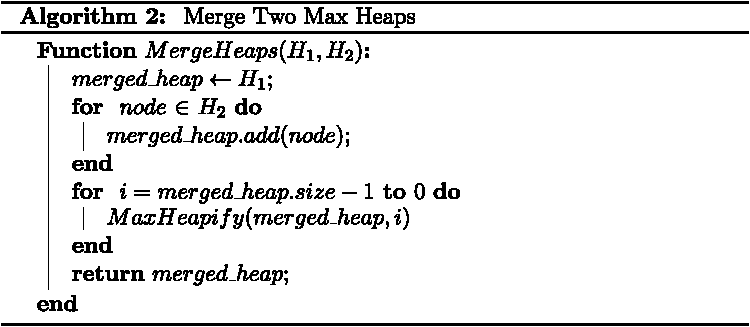
\includegraphics{Render-Task2}
    \end{figure}
\end{solution}


\begin{problem}
    \textbf{Исправление рассказанного в лекции \texttt{merge} для скошенных влево куч}.
    Реализация, рассказанная на лекции, выглядит примерно так:

    {
        \normalfont\begin{lstlisting}
node *merge(node *h1, node *h2) {
    if (h1 == nullptr) return h2;
    if (h2 == nullptr) return h1;

    h1->right = merge(h1->right, h2);

    if (h1->left->rank < h1->right->rank)
        swap(h1->left, h1->right);
    h1->rank = h1->right->rank + 1;
    return h1;
}
        \end{lstlisting}
    }

    Иными словами, мы спускаемся до ближайшего свободного места в \texttt{h1}, подвешиваем туда \texttt{h2}, после чего
    при подъеме обратно меняем местами левого и правого ребенка и пересчитываем \texttt{rank} вершин при необходимости.

    Как можно заметить, такая реализация работает только если все элементы в куче \texttt{h2} больше определенных
    элементов в \texttt{h1}. Модифицируйте реализацию так, чтобы она стала корректной вне зависимости от отношений
    между элементами \texttt{h1} и \texttt{h2} (время работы должно остаться $O(n \log n)$. \\
    {\footnotesize Визуализацию можно посмотреть \href{https://www.cs.usfca.edu/~galles/visualization/LeftistHeap.html}{здесь}}
\end{problem}

\begin{solution}
    \medskip\noindent

    \begin{lstlisting}
node* merge(node* h1, node* h2)
{
    if (!h1)
    {
        return h2;
    }

    if (!h2)
    {
        return h1;
    }

    if (h1->value < h2->value)
    {
        return merge_internal(h1, h2);
    }
    else
    {
        return merge_internal(h2, h1);
    }
}

static node* merge_internal(node* h1, node* h2)
{
    if (!h1->left)
    {
        h1->left = h2;
    }
    else
    {
        h1->right = merge(h1->right, h2);

        if (h1->left->rank < h1->right->rank)
        {
            std::swap(h1->left, h1->right);
        }

        h1->rank = h1->right->rank + 1;
    }

    return h1;
}
    \end{lstlisting}
\end{solution}


\begin{problem}
    Опишите структуру данных, реализующую следующие операции:
    \begin{itemize}
        \item \texttt{push(key, priority)}~-- добавить ключ \texttt{key} (которого там не было) с приоритетом \texttt{priority}.
        \item \texttt{pop()}~-- извлечь ключ с минимальным приоритетом.
        \item \texttt{decrease\_priority(key, new\_priority)}~-- уменьшить приоритет ключа \texttt{key} (который в этот момент присутствует в структуре).
    \end{itemize}
    Все ключи~-- целые числа от 1 до $n$. Все операции должны работать за $O(\log{n})$.
\end{problem}

\begin{solution}
    \medskip\noindent

    Эта структура~-- индексированная очередь с приоритетами. Это та же очередь с приоритетами на базе кучи,
    только дополнительно строится хэш-мапа для установления соотношения между ключом и индексом в контейнере,
    а в сам контейнер помещаются пары ключ-приоритет.

    Все вышеперечисленные операции в этой структуре работают за $O(\log{n})$.
\end{solution}


\subsection*{Дополнительные задачи}

\begin{problem}
    Для корректной реализации \texttt{LeftistHeap} (которая позволяет сливать любые две кучи, см. визуализатор выше):
    \begin{enumerate}[a)]
        \item докажите, что время работы операции $\mathtt{DecreaseKey}(i, x)$~-- это $O(\log n)$ \\
            {
                \footnotesize \textbf{Подсказка}: докажите, что при каждом подъеме, при котором мы меняем детей местами,
                $\mathtt{rank}(v)$ увеличивается хотя бы на $1$.
            }
        \item придумайте работающий за $O(n)$ \texttt{BuildHeap()} для скошенной влево кучи
    \end{enumerate}
\end{problem}

\begin{solution}
    \dots
\end{solution}


\begin{problem}
    Куча хранится в массиве $h$ длины $n$. Родитель $p$ хранит детей в ячейках $2 \cdot p + 1$ и $2 \cdot p + 2$.
    Алгоритм приступает к сортировке. Сортировка $n$ раз выполняет следующие действия:
    \begin{itemize}
        \item Поменять первый и последний элемент кучи местами.
        \item Уменьшить $n$ на единицу.
        \item Запустить \texttt{SiftDown} на первом элементе.
    \end{itemize}

    {
        \normalfont\begin{lstlisting}
void SiftDown(int i) {
    int j = 2 * i + 1;
    if (j + 1 < n && h[j + 1] > h[j])
        j = j + 1;
    if (j < n && h[j] > h[i]) {
        swap(h[i], h[j]);
        SiftDown(j);
    }
}
        \end{lstlisting}
    }

    Придумайте алгоритм, который по $n$ выдаёт перестановку чисел от $1$ до $n$, которая является корректной кучей
    и приводит к максимальному количеству вызовов \texttt{SiftDown} при сортировке. Время работы~-- $O(n \log n)$.
\end{problem}

\begin{solution}
    \dots
\end{solution}


\clearpage
